%\documentclass[hyperref={pdfpagelabels=false},slidetop,9pt]{beamer}
\documentclass[slidetop,8pt]{beamer}
\usepackage[T1]{fontenc}
\usepackage[utf8]{inputenc}
\newcommand{\id}{30}
\newcommand{\nom}{Calculs d'hyperstatisme}
\newcommand{\sequence}{04}
\newcommand{\nomsequence}{Liaisons entre les solides}
\newcommand{\num}{03}
\newcommand{\type}{TD}
\newcommand{\descrip}{En appliquant les règles de la théorie des mécanisme, déterminer le degré d'hyperstatisme de plusieurs systèmes et proposer des solutions afin de diminuer ce degré}
\newcommand{\competences}{B2-12: Proposer une modélisation des liaisons avec leurs caractéristiques géométriques. \\ &  B2-13: Proposer un modèle cinématique paramétré à partir d'un système réel, d'une maquette numérique ou d'u \\ &  B2-17: Simplifier un modèle de mécanisme. \\ &  B2-18: Modifier un modèle pour le rendre isostatique.}
\newcommand{\nbcomp}{4}
\newcommand{\systemes}{E.P.A.S, Machine d'essai de traction}
\newcommand{\systemesnum}{14, 13}
\newcommand{\systemessansaccent}{E.P.A.S, Machine d'essai de traction}
\newcommand{\ilot}{3}
\newcommand{\ilotstr}{03}
\newcommand{\dossierilot}{\detokenize{Ilot_03 E.P.A.S, Machine d'essai de traction}}
\newcommand{\imageun}{EPAS}
\newcommand{\imagedeux}{Machine_dessai_de_traction}

\usepackage{etex}
\usepackage{tikz}
\usepackage[european]{circuitikz}
\usepackage{pgf}
\usepackage[all]{xy}
\usepackage{pgfpages}
\usepackage{graphbox}
\usepackage{pdfpages}
%\usepackage[adobe-utopia]{mathdesign}
\usepackage{ifthen}
\usepackage{cancel}
\usepackage{framed}
\usepackage{subfig}
\usepackage{tabularx}
\usepackage{setspace}
\usepackage{soul}
\usepackage{schemabloc}
\usepackage{eqnarray}
\usepackage[dot, phantomtext]{dashundergaps}
\usepackage{media9}
\usepackage{multimedia}
\usepackage{textcomp}
\usefonttheme[onlymath]{serif}

\author{Renaud Costadoat}
\institute{Lycée Dorian}

\usepackage{multido}
\usepackage{multirow}
\usepackage{multicol} % Portions de texte en colonnes
\usepackage{flafter}%floatants après la référence

\usepackage{color}
\usepackage{xcolor}
\usepackage{colortbl}

\usepackage[gen]{eurosym}
\usepackage{tikz}
%\usepackage{pstricks,pst-node,pst-tree,pst-solides3d}
\usepackage{lmodern}
\usepackage[francais]{babel}
\usepackage{pslatex}
\usetheme{renaud}
\usepackage{times}
\usepackage[frenchmath]{newtxsf} % for sans serif symbols
\renewcommand{\familydefault}{\sfdefault}
%\usepackage{amsfonts}
%\usepackage{amsmath}
%\usepackage{mathastext}
\usepackage{verbatim}
\usepackage{moreverb}
%\usetikzlibrary{arrows,shapes}
\usepackage{graphicx}
\usepackage{psfrag}
\usepackage{wrapfig}
\usepackage{etoolbox}

\definecolor{gris25}{gray}{0.75}
\definecolor{bleu}{RGB}{18,33,98}
\definecolor{bleuf}{RGB}{42,94,171}
\definecolor{bleuc}{RGB}{231,239,247}
\definecolor{rougef}{RGB}{185,18,27}
\definecolor{rougec}{RGB}{255,188,204}%255,230,231
\definecolor{vertf}{RGB}{103,126,82}
\definecolor{vertc}{RGB}{220,255,191}

\setlength\parindent{24pt}
\parskip 7.2pt
\parindent 8pt

\newenvironment{rem}[1][\hsize]%
{%
    \def\FrameCommand
   {%
\rotatebox{90}{\textit{\textsf{Remarque}}} 
       {\color{bleuf}\vrule width 3pt}%
       \hspace{0pt}%must no space.
       \fboxsep=\FrameSep\colorbox{bleuc}%
  }%
    \MakeFramed{\hsize#1\advance\hsize-\width\FrameRestore}%
}%
{\endMakeFramed}%


\newenvironment{savoir}[1][\hsize]%
{%
    \def\FrameCommand
    {%
\rotatebox{90}{\textit{\textsf{Savoir}}} 
        {\color{bleuf}\vrule width 3pt}%
        \hspace{0pt}%must no space.
        \fboxsep=\FrameSep\colorbox{bleuc}%
    }%
    \MakeFramed{\hsize#1\advance\hsize-\width\FrameRestore}%
}%
{\endMakeFramed}%

\newenvironment{prob}[1][\hsize]%
{%
    \def\FrameCommand%
    {%
\rotatebox{90}{\textit{\textsf{Problematique}}} 
        {\color{rougef}\vrule width 3pt}%
        \hspace{0pt}%must no space.
        \fboxsep=\FrameSep\colorbox{rougec}%
    }%
    \MakeFramed{\hsize#1\advance\hsize-\width\FrameRestore}%
}%
{\endMakeFramed}%

\newenvironment{obj}[1][\hsize]%
{%
    \def\FrameCommand%
    {%
\rotatebox{90}{\textit{\textsf{Objectif}}} 
        {\color{vertf}\vrule width 3pt}%
        \hspace{0pt}%must no space.
        \fboxsep=\FrameSep\colorbox{vertc}%
    }%
    \MakeFramed{\hsize#1\advance\hsize-\width\FrameRestore}%
}%
{\endMakeFramed}%

\newenvironment{defi}[1][\hsize]%
{%
    \def\FrameCommand%
    {%
\rotatebox{90}{\textit{\textsf{Definition}}} 
        {\color{bleuf}\vrule width 3pt}%
        \hspace{0pt}%must no space.
        \fboxsep=\FrameSep\colorbox{rougec}%
    }%
    \MakeFramed{\hsize#1\advance\hsize-\width\FrameRestore}%
}%
{\endMakeFramed}%


\newenvironment{hypo}[1][\hsize]%
{%
    \def\FrameCommand%
    {%
\rotatebox{90}{\textit{\textsf{Hypothèse\\}}} 
        {\color{bleuf}\vrule width 3pt}%
        \hspace{0pt}%must no space.
        \fboxsep=\FrameSep\colorbox{bleuc}%
    }%
    \MakeFramed{\hsize#1\advance\hsize-\width\FrameRestore}%
}%
{\endMakeFramed}%


\newenvironment{prop}[1][\hsize]%
{%
    \def\FrameCommand%
    {%
\rotatebox{90}{\textit{\textsf{Propriété}}} 
        {\color{bleuf}\vrule width 3pt}%
        \hspace{0pt}%must no space.
        \fboxsep=\FrameSep\colorbox{bleuc}%
    }%
    \MakeFramed{\hsize#1\advance\hsize-\width\FrameRestore}%
}%
{\endMakeFramed}%

\newenvironment{props}[1][\hsize]%
{%
    \def\FrameCommand%
    {%
\rotatebox{90}{\textit{\textsf{Propriétés}}} 
        {\color{bleuf}\vrule width 3pt}%
        \hspace{0pt}%must no space.
        \fboxsep=\FrameSep\colorbox{bleuc}%
    }%
    \MakeFramed{\hsize#1\advance\hsize-\width\FrameRestore}%
}%
{\endMakeFramed}%

\newenvironment{exemple}[1][\hsize]%
{%
    \def\FrameCommand%
    {%
\rotatebox{90}{\textit{\textsf{Exemple}}} 
        {\color{vertf}\vrule width 3pt}%
        \hspace{0pt}%must no space.
        \fboxsep=\FrameSep\colorbox{vertc}%
    }%
    \MakeFramed{\hsize#1\advance\hsize-\width\FrameRestore}%
}%
{\endMakeFramed}%

\newenvironment{resultat}[1][\hsize]%
{%
    \def\FrameCommand%
    {%
\rotatebox{90}{\textit{\textsf{Résultat}}} 
        {\color{rougef}\vrule width 3pt}%
%        {\color{bleuf}\vrule width 3pt}%
        \hspace{0pt}%must no space.
        \fboxsep=\FrameSep\colorbox{rougec}%
    }%
    \MakeFramed{\hsize#1\advance\hsize-\width\FrameRestore}%
}%
{\endMakeFramed}%

\newenvironment{methode}[1][\hsize]%
{%
    \def\FrameCommand%
    {%
\rotatebox{90}{\textit{\textsf{Méthode\\}}} 
        {\color{rougef}\vrule width 3pt}%
        \hspace{0pt}%must no space.
        \fboxsep=\FrameSep\colorbox{rougec}%
    }%
    \MakeFramed{\hsize#1\advance\hsize-\width\FrameRestore}%
}%
{\endMakeFramed}%

\newenvironment{theo}[1][\hsize]%
{%
    \def\FrameCommand%
    {%
\rotatebox{90}{\textit{\textsf{Théorème\\}}} 
        {\color{rougef}\vrule width 3pt}%
        \hspace{0pt}%must no space.
        \fboxsep=\FrameSep\colorbox{rougec}%
    }%
    \MakeFramed{\hsize#1\advance\hsize-\width\FrameRestore}%
}%
{\endMakeFramed}%

\newenvironment{warn}[1][\hsize]%
{%
    \def\FrameCommand%
    {%
\rotatebox{90}{\textit{\textsf{Attention\\}}} 
        {\color{rougef}\vrule width 3pt}%
        \hspace{0pt}%must no space.
        \fboxsep=\FrameSep\colorbox{rougec}%
    }%
    \MakeFramed{\hsize#1\advance\hsize-\width\FrameRestore}%
}%
{\endMakeFramed}%

% \usepackage{pstricks}
%\usepackage{minitoc}
% \setcounter{minitocdepth}{4}

\setcounter{tocdepth}{2}

% \mtcselectlanguage{french} 

%\usepackage{draftcopy}% "Brouillon"
% \usepackage{floatflt}
\usepackage{psfrag}
%\usepackage{listings} % Permet d'insérer du code de programmation
\renewcommand{\baselinestretch}{1.2}

% Changer la num�rotation des figures :
% ------------------------------------
% \makeatletter
% \renewcommand{\thefigure}{\ifnum \c@section>\z@ \thesection.\fi
%  \@arabic\c@figure}
% \@addtoreset{figure}{section}
% \makeatother
 


%%%%%%%%%%%%
% Définition des vecteurs %
%%%%%%%%%%%%
 \newcommand{\vect}[1]{\overrightarrow{#1}}

%%%%%%%%%%%%
% Définition des torseusr %
%%%%%%%%%%%%

 \newcommand{\torseur}[1]{%
\left\{{#1}\right\}
}

\newcommand{\torseurcin}[3]{%
\left\{\mathcal{#1} \left(#2/#3 \right) \right\}
}

\newcommand{\torseurstat}[3]{%
\left\{\mathcal{#1} \left(#2\rightarrow #3 \right) \right\}
}

 \newcommand{\torseurc}[8]{%
%\left\{#1 \right\}=
\left\{
{#1}
\right\}
 = 
\left\{%
\begin{array}{cc}%
{#2} & {#5}\\%
{#3} & {#6}\\%
{#4} & {#7}\\%
\end{array}%
\right\}_{#8}%
}

 \newcommand{\torseurcol}[7]{
\left\{%
\begin{array}{cc}%
{#1} & {#4}\\%
{#2} & {#5}\\%
{#3} & {#6}\\%
\end{array}%
\right\}_{#7}%
}

 \newcommand{\torseurl}[3]{%
%\left\{\mathcal{#1}\right\}_{#2}=%
\left\{%
\begin{array}{l}%
{#1} \\%
{#2} %
\end{array}%
\right\}_{#3}%
}

 \newcommand{\vectv}[3]{%
\vect{V\left( {#1} \in {#2}/{#3}\right)}
}


\newcommand{\vectf}[2]{%
\vect{R\left( {#1} \rightarrow {#2}\right)}
}

\newcommand{\vectm}[3]{%
\vect{\mathcal{M}\left( {#1}, {#2} \rightarrow {#3}\right)}
}


 \newcommand{\vectg}[3]{%
\vect{\Gamma \left( {#1} \in {#2}/{#3}\right)}
}

 \newcommand{\vecto}[2]{%
\vect{\Omega\left( {#1}/{#2}\right)}
}

\newcommand{\reponse}[1][4]
{
\multido{}{#1}
{
\begin{center}
\makebox[0.9\linewidth]{\dotfill} \end{center}
}}


% }$$\left\{\mathcal{#1} \right\}_{#2} =%
% \left\{%
% \begin{array}{c}%
%  #3 \\%
%  #4 %
% \end{array}%
% \right\}_{#5}}


%  ------------------------------------------
% | Modification du formatage des sections : | 
%  ------------------------------------------

% Grands titres :
% ---------------

\newcommand{\titre}[1]{%
\begin{center}
      \bigskip
      \rule{\textwidth}{1pt}
      \par\vspace{0.1cm}
      
      \textbf{\large #1}
      \par\rule{\textwidth}{1pt}
    \end{center}
    \bigskip
  }

% Supprime le numéro du chapitre dans la numérotation des sections:
% -----------------------------------------------------------------
\makeatletter
\renewcommand{\thesection}{\@arabic\c@section}
\makeatother


% \titleformat{\chapter}[display]
% {\normalfont\Large\filcenter}
% {}
% {1pc}
% {\titlerule[1pt]
%   \vspace{1pc}%
%   \Huge}[\vspace{1ex}%
% \titlerule]


%%%% Chapitres Comme PY Pechard %%%%%%%%%
% numéro du chapitre
\DeclareFixedFont{\chapnumfont}{OT1}{phv}{b}{n}{80pt}
% pour le mot " Chapitre "
\DeclareFixedFont{\chapchapfont}{OT1}{phv}{m}{it}{40pt}
% pour le titre
\DeclareFixedFont{\chaptitfont}{T1}{phv}{b}{n}{25pt}

\definecolor{gris}{gray}{0.75}
\setbeamertemplate{section in toc}[sections numbered]

\newlength{\RoundedBoxWidth}
\newsavebox{\GrayRoundedBox}
\newenvironment{GrayBox}[1][\dimexpr\textwidth-4.5ex]%
   {\setlength{\RoundedBoxWidth}{\dimexpr#1}
    \begin{lrbox}{\GrayRoundedBox}
       \begin{minipage}{\RoundedBoxWidth}}%
   {   \end{minipage}
    \end{lrbox}
    \begin{center}
    \begin{tikzpicture}%
       \draw node[draw=bleuf,fill=bleuc,rounded corners,%
             inner sep=2ex,text width=\RoundedBoxWidth]%
             {\usebox{\GrayRoundedBox}};
    \end{tikzpicture}
    \end{center}}
    
\ifdef{\prive}{\pgfpagesuselayout{2 on 1}[a4paper,border shrink=0mm]}
\ifdef{\prive}{\setbeamertemplate{navigation symbols}{}}
\setbeamertemplate{itemize item}[ball]
%\setbeamertemplate{blocks}[rounded]%[shadow=true]
\setbeamercolor{block title}{fg=white,bg=grisf}        % titre block normal 
\setbeamercolor{block body}{fg=grisf,bg=grisc!50}      % corps block normal
\setbeamercolor{block body alerted}{fg=white,bg=warning}   % idem pour un block alerte

\title{\nom}
\date{S\sequence \ - \type\num}

\begin{document}
\shorthandoff{:!}
\bibliographystyle{abbrvnat-fr}

\usebackgroundtemplate%
{%
    \centering\includegraphics[width=\paperwidth]{/home/renaud/Documents/Renaud/GitHub/Sciences-Ingenieur/img/fond2}%
}

{
\setbeamertemplate{navigation symbols}{}
\setbeamertemplate{headline}[pagetitre]
\setbeamertemplate{footline}[pagetitre]
\usebackgroundtemplate{\centering\includegraphics[width=\paperwidth]{/home/renaud/Documents/Renaud/GitHub/Sciences-Ingenieur/img/fond}}
\frame{\titlepage}
}



\section{Introduction}

{\frame{
\frametitle{Introduction}

\begin{savoir}
Vous êtes capables :
\begin{itemize}
 \item de représenter une liaison pivot sur un schéma cinématique,
 \item de modéliser la liaison pivot par un torseur cinématique,
 \item de décomposer architecturalement une liaison pivot. 
\end{itemize}
\end{savoir}

\begin{prob}
Vous devez êtes capables :
 \begin{itemize}
 \item de concevoir un guidage en liaison pivot,
 \item de donner des caractéristiques techniques sur ce guidage.
 \end{itemize}
\end{prob}
}}

{\frame{
\frametitle{Exigences d'une liaison pivot}

Une liaison pivot doit être conçue en prenant en compte les besoins du cahier des charges. Le choix de la réalisation de la liaison pivot doit être fait en prenant en répondant aux trois exigences représentées sur le diagramme suivant.

\vfill

\begin{center}
	\includegraphics[width=0.8\linewidth]{img/Exigences_1}
\end{center}
}}

{\frame{
\frametitle{Le contact direct}

\begin{minipage}{0.6\linewidth}
Le \textbf{contact direct} ainsi que les \textbf{coussinets} permettent un guidage de \textit{faible qualité}.

Caractéristiques :
\begin{itemize}
 \item vitesse de rotation faible,
 \item efforts moyens.
\end{itemize}

\end{minipage}\hfill
\begin{minipage}{0.35\linewidth}
	\includegraphics[width=0.8\linewidth]{img/Exigences_2}
\end{minipage}

\begin{minipage}{0.35\linewidth}
	\includegraphics[width=0.8\linewidth]{img/Direct}
\end{minipage}\hfill
\begin{minipage}{0.6\linewidth}
\textbf{Contact direct:} La qualité du contact direct dépend directement du \textbf{matériau} et de la qualité de surface des pièces en contact ainsi que du \textbf{lubrifiant} qui peut être disposé entre les deux.
\end{minipage}
}}

{\frame{
\frametitle{Les coussinets}

\begin{minipage}{0.6\linewidth}
Un \textbf{coussinet} est un élément qui s'insère entre les deux pièces en rotation afin de \textbf{diminuer les frottements}. Le matériau des coussinets (\textbf{bronze}, PTFE,...) favorise le glissement.

Le \textbf{bronze}, par exemple, est utilisé pour sa \textbf{porosité} qui retient le lubrifiant. Afin de minimiser le frottement, le coussinet sera toujours monté serré (pas de glissement) avec l'alésage.
\end{minipage}\hfill
\begin{minipage}{0.35\linewidth}
	\includegraphics[width=0.8\linewidth]{img/Coussinet}
\end{minipage}

La vitesse de glissement n'excèdera pas \textbf{quelques mètres par seconde}. Les efforts ayant tendance à écraser le coussinet, ils devront être limités.
}}

{\frame{
\frametitle{Les coussinets}

\begin{minipage}{0.7\linewidth}
Les coussinets sont montés entre l'arbre et l'alésage. Des coussinets sont équipés d'une \textbf{collerette} afin de gérer les efforts axiaux.

La figure ci-dessous montre le \textbf{montage de coussinets} mis en place sur le système Maxpid.
\end{minipage}\hfill
\begin{minipage}{0.25\linewidth}
	\includegraphics[width=0.8\linewidth]{img/Coussinet_col}
\end{minipage}

\vfill

\begin{center}
	\includegraphics[width=0.6\linewidth]{img/Montage_coussinet}
\end{center}


}}

{\frame{
\frametitle{Les roulements}

\begin{minipage}{0.6\linewidth}
Un \textbf{roulement} permet un guidage de \textit{bonne qualité}.

Caractéristiques :
\begin{itemize}
 \item vitesse de rotation importantes,
 \item efforts importants.
\end{itemize}

Le choix d'un \textbf{roulement} dépend de la nature (direction, norme,...) des efforts transitant par la liaison.

\vspace{1cm}

\begin{minipage}{0.45\linewidth}
	\includegraphics[width=0.9\linewidth]{img/Rlt_billes}
\end{minipage}\hfill
\begin{minipage}{0.4\linewidth}
	\includegraphics[width=0.9\linewidth]{img/Rlt_rouleaux}
\end{minipage}
\end{minipage}\hfill
\begin{minipage}{0.35\linewidth}
	\includegraphics[width=0.9\linewidth]{img/Exigences_3}
\end{minipage}
}}

{\frame{
\frametitle{Constitution d'un roulement}

\begin{minipage}{0.6\linewidth}
Les constituants d'un roulement sont:
\begin{itemize}
 \item Une \textbf{bague extérieure} en contact avec l'alésage,
 \item Une \textbf{bague intérieure} en contact avec l'arbre,
 \item Des \textbf{éléments roulants} (billes, rouleaux ou aiguilles),
 \item Une \textbf{cage} permettant de maintenir les éléments roulants en place.
\end{itemize}
\end{minipage}\hfill
\begin{minipage}{0.3\linewidth}
	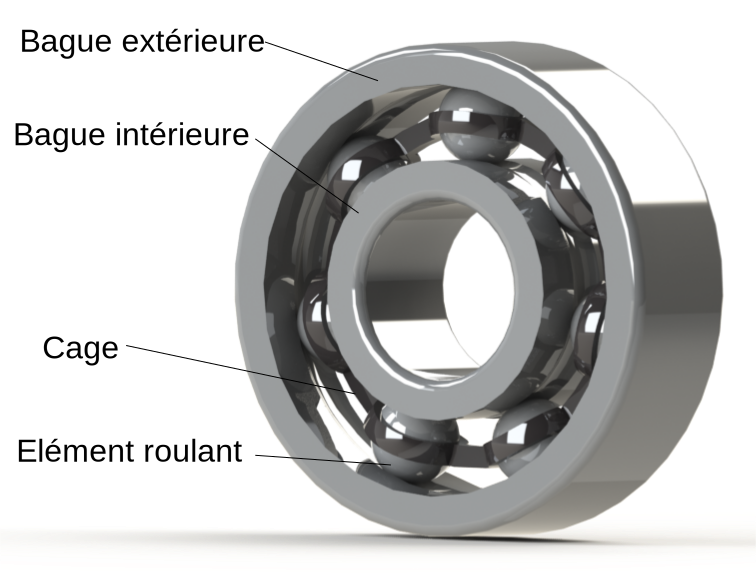
\includegraphics[width=0.9\linewidth]{img/Rlt_constituants}
\end{minipage}

}}

{\frame{
\frametitle{Les roulements à billes}

\begin{minipage}{0.6\linewidth}
Les zones de contact entre les billes et les bagues étant de faible surface (points), les contraintes deviennent très importantes lorsque des efforts sont appliqués.
\begin{itemize}
 \item Efforts radiaux moyens,
 \item Efforts axiaux faibles.
\end{itemize}
\end{minipage}\hfill
\begin{minipage}{0.3\linewidth}
	\includegraphics[width=0.9\linewidth]{img/Exigences_6}
\end{minipage}

\vfill

\begin{center}
	\includegraphics[height=2cm]{img/Picture1} \hspace{0.5cm}
		\includegraphics[height=2cm]{img/Picture2}
\end{center}
}}

{\frame{
\frametitle{Les roulements à rouleaux}

\begin{minipage}{0.5\linewidth}
Les zones de contact entre les rouleaux et les bagues étant de plus grandes surfaces (lignes), des efforts plus importantes peuvent être appliqués.
\begin{itemize}
 \item Efforts radiaux élevés,
 \item Efforts axiaux nuls.
\end{itemize}


\end{minipage}\hfill
\begin{minipage}{0.45\linewidth}
	\includegraphics[width=0.9\linewidth]{img/Exigences_7}
\end{minipage}

\vfill

\begin{center}
	\includegraphics[height=2cm]{img/Picture3} \hspace{0.5cm}
		\includegraphics[height=2cm]{img/Picture4}
\end{center}
}}

{\frame{
\frametitle{Les roulements à aiguilles}

\begin{minipage}{0.5\linewidth}
Les aiguilles sont équivalentes à des rouleaux de faible diamètre. De plus les roulements à aiguilles ne possèdent en général pas de bague intérieur. Cela permet de diminuer grandement l'encombrement.
\begin{itemize}
 \item Efforts radiaux élevés,
 \item Efforts axiaux nuls.
\end{itemize}
\end{minipage}\hfill
\begin{minipage}{0.45\linewidth}
	\includegraphics[width=0.9\linewidth]{img/Exigences_8}
\end{minipage}

\vfill

\begin{center}
		\includegraphics[height=4cm]{img/Picture5}
\end{center}

}}

{\frame{
\frametitle{Les butée à billes}

\begin{minipage}{0.5\linewidth}
Les butées à billes sont l'équivalent de roulements ayant l'axe des points de contact entre les billes et les bagues dirigé axialement.
\begin{itemize}
 \item Efforts radiaux nuls,
 \item Efforts axiaux élevés.
\end{itemize}
\end{minipage}\hfill
\begin{minipage}{0.45\linewidth}
	\includegraphics[width=0.9\linewidth]{img/Exigences_9}
\end{minipage}

\vfill

\begin{center}
		\includegraphics[height=3cm]{img/Picture7}
\end{center}
}}

{\frame{
\frametitle{Les montages de roulements}

\begin{center}
		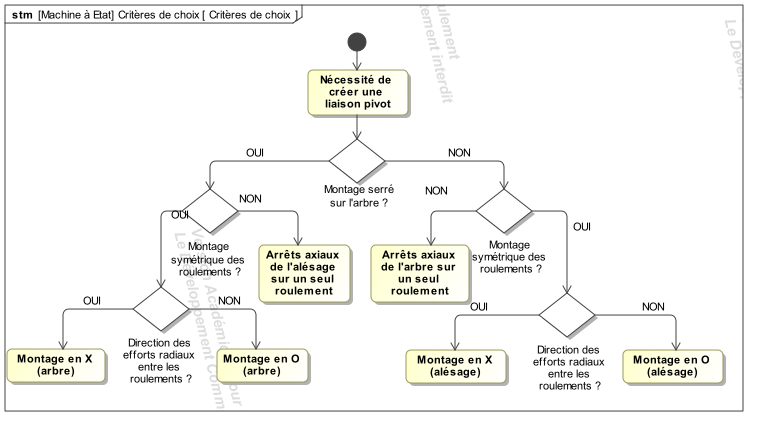
\includegraphics[width=0.9\linewidth]{img/Criteres_de_choix.pdf}
\end{center}

}}

{\frame{
\frametitle{Les montages de roulements}

\textbf{Roulements serrés sur l'arbre}

\hfill\begin{minipage}{0.28\linewidth} \centering Roulement privilégié \end{minipage} \hfill \begin{minipage}{0.28\linewidth} \centering Montage en X \end{minipage} \hfill
\begin{minipage}{0.28\linewidth} \centering Montage en O \end{minipage} \hfill ~\

\begin{center}
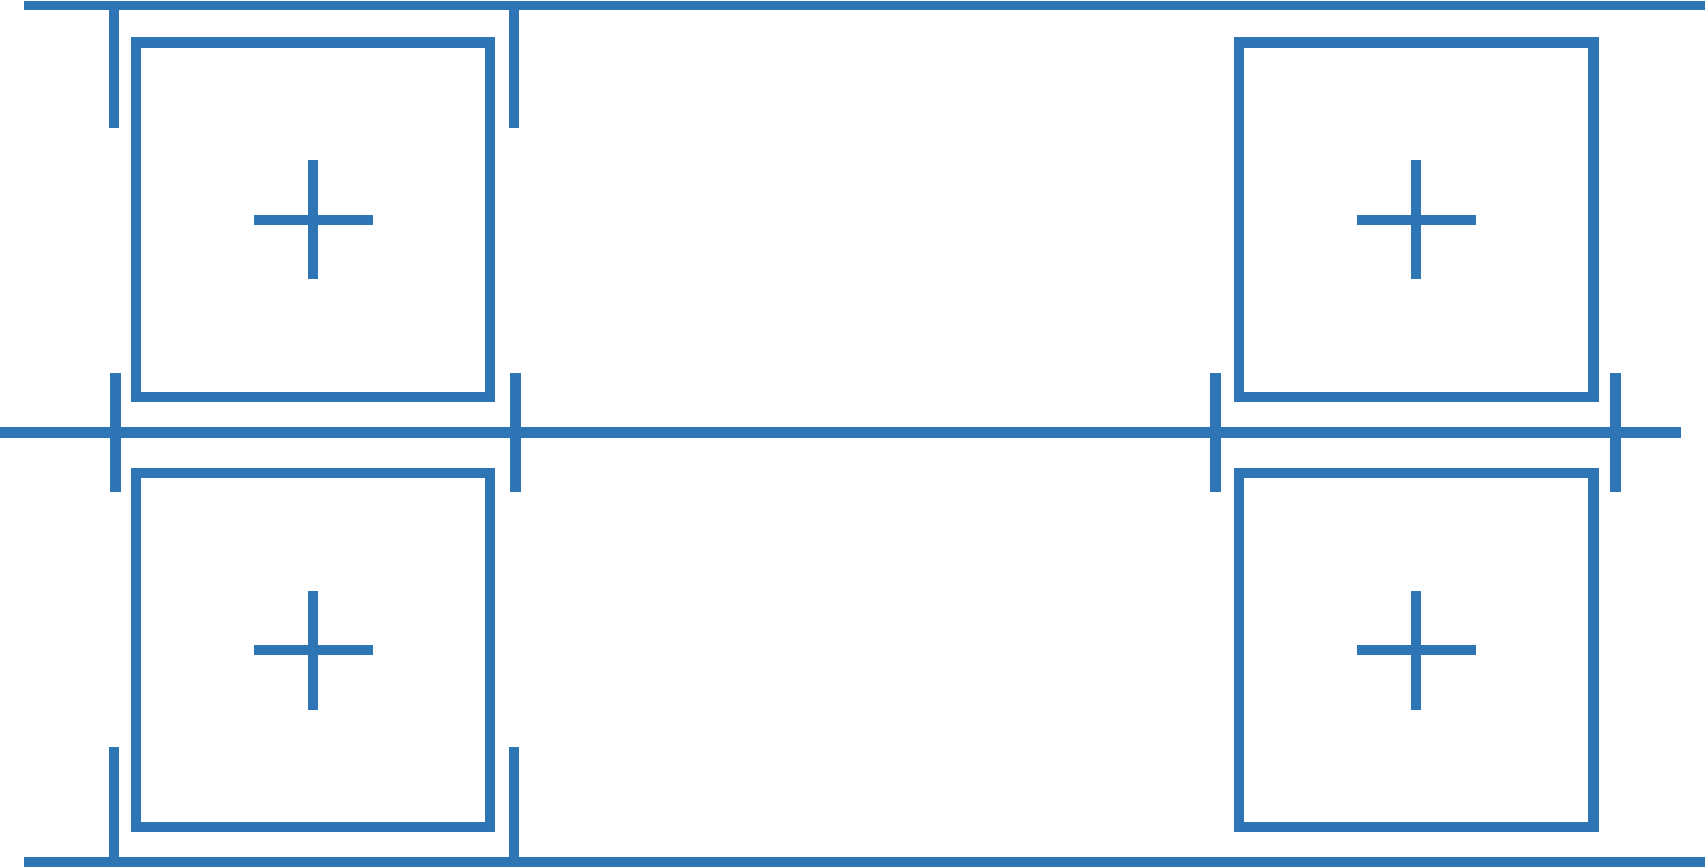
\includegraphics[width=0.3\linewidth]{img/Modele_1.pdf}
\includegraphics[width=0.3\linewidth]{img/Modele_2.pdf}
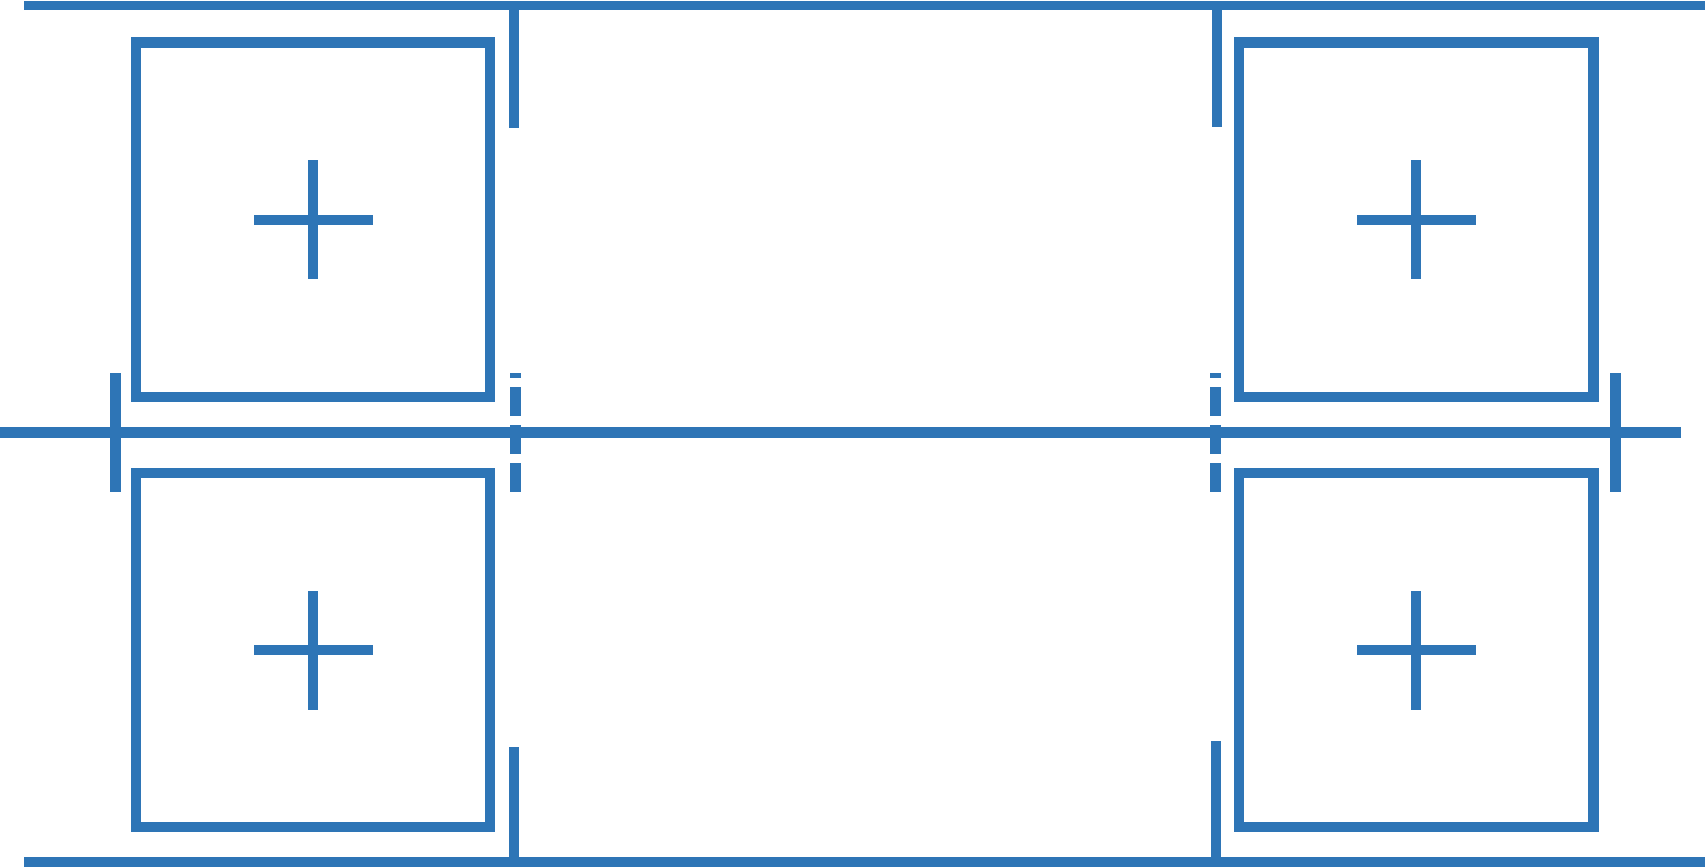
\includegraphics[width=0.3\linewidth]{img/Modele_3.pdf}
\end{center}

\textbf{Roulements serrés sur l'alésage}

\hfill\begin{minipage}{0.28\linewidth} \centering Roulement privilégié \end{minipage} \hfill \begin{minipage}{0.28\linewidth} \centering Montage en X \end{minipage} \hfill
\begin{minipage}{0.28\linewidth} \centering Montage en O \end{minipage} \hfill ~\

\begin{center}
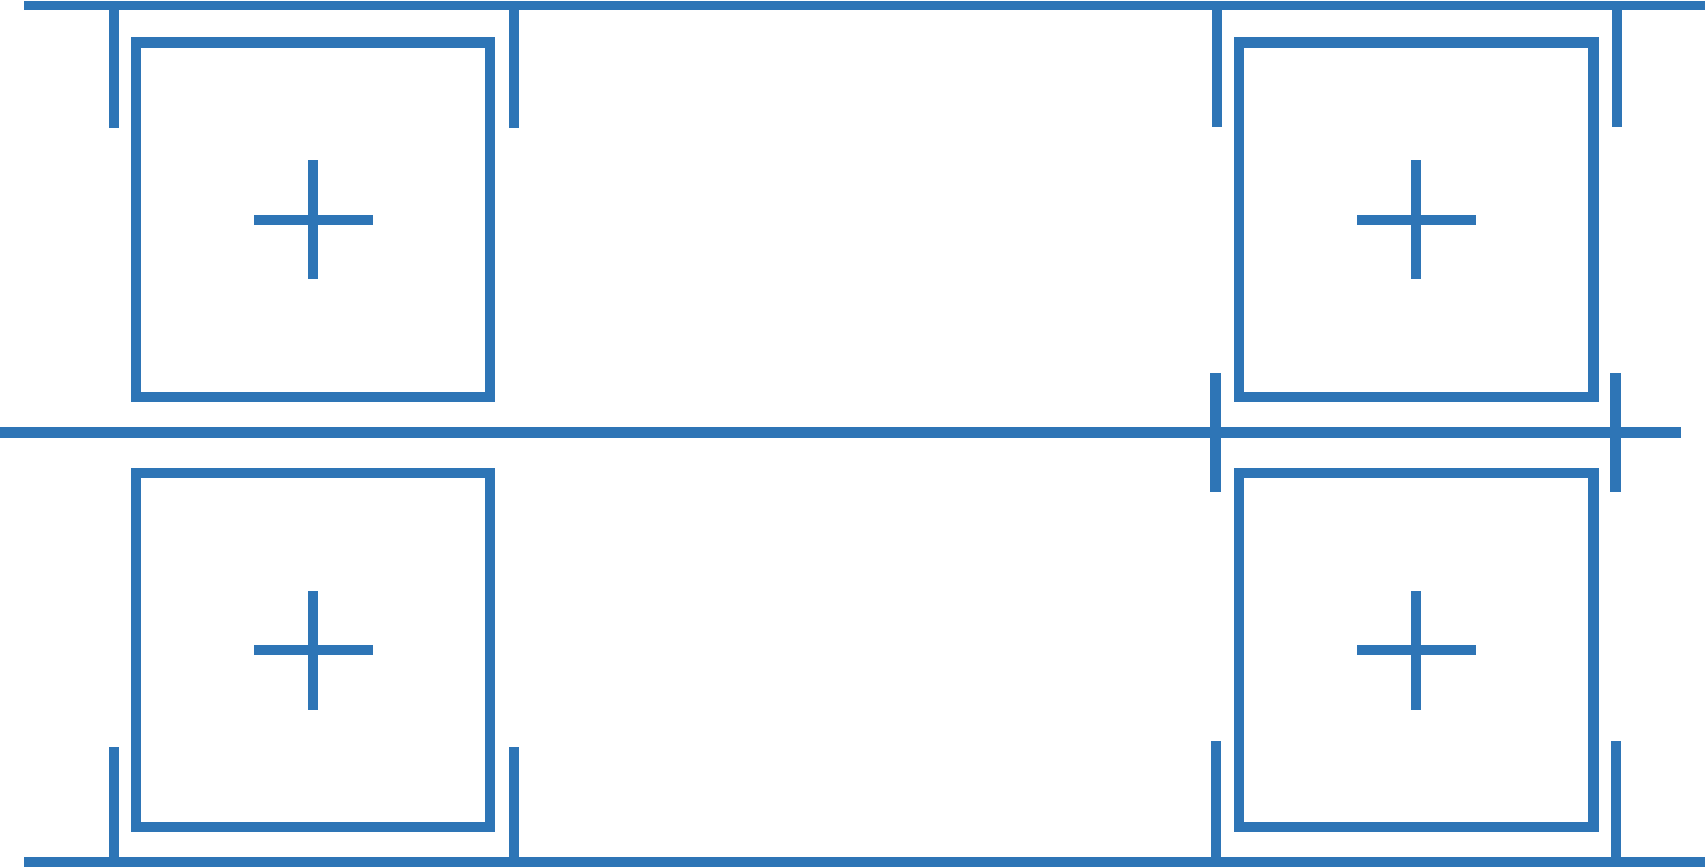
\includegraphics[width=0.3\linewidth]{img/Modele_4.pdf}
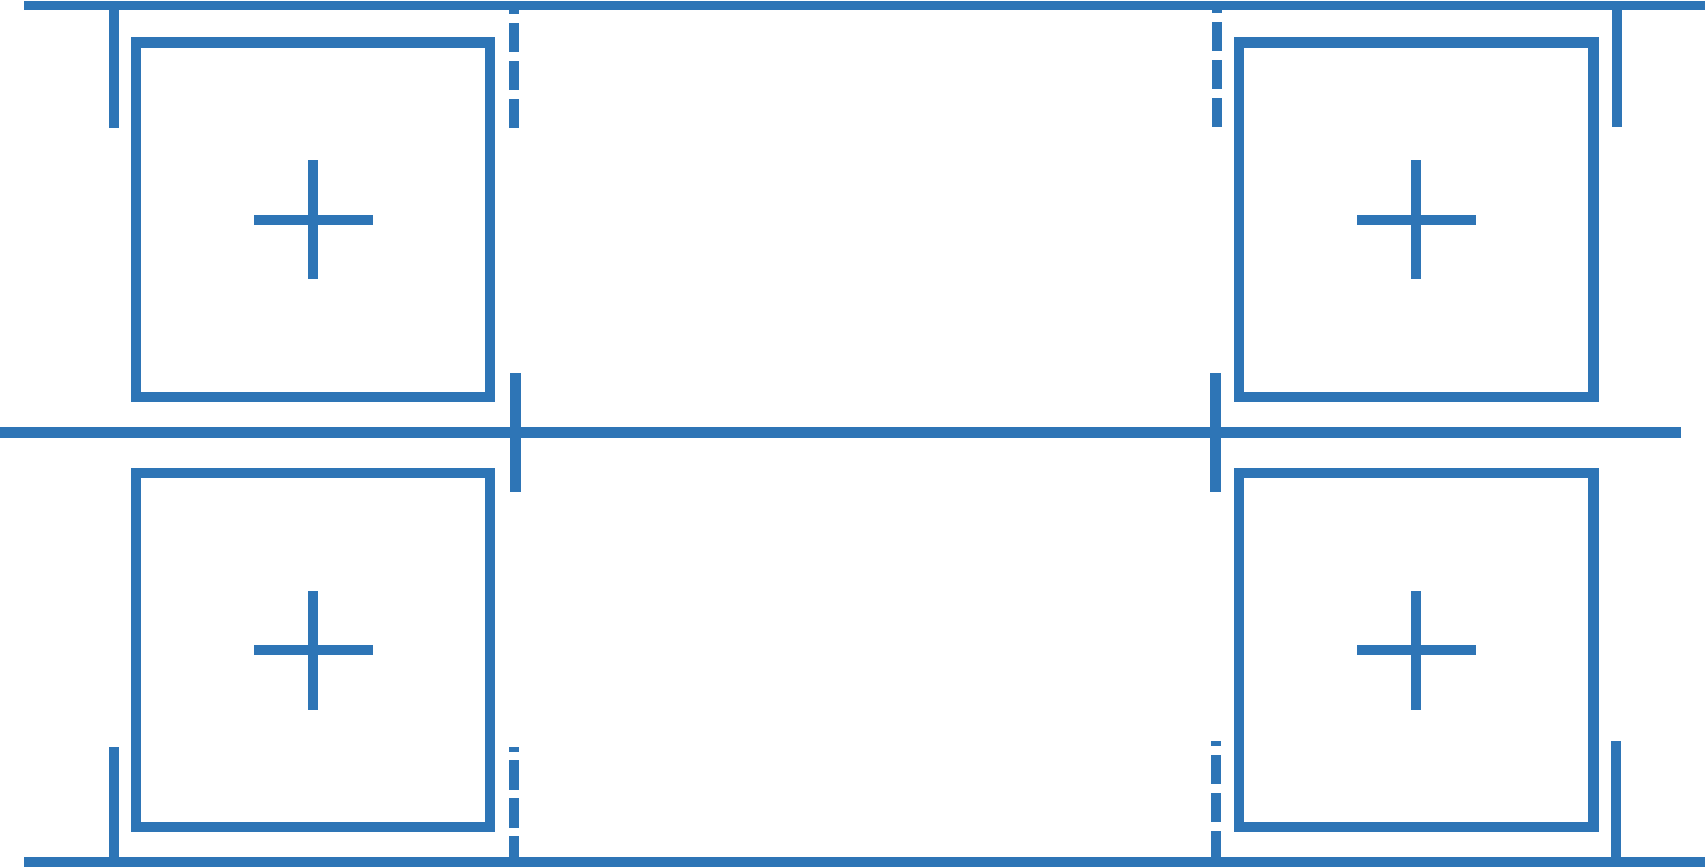
\includegraphics[width=0.3\linewidth]{img/Modele_6.pdf}
\includegraphics[width=0.3\linewidth]{img/Modele_5.pdf}
\end{center}
}}

{\frame{
\frametitle{Les montages de roulements}

\begin{rem}
Dans le cas d'un montage en X ou en O sans les arrêt facultatifs, il est impossible de différencier un montage serré sur l'arbre ou serré sur l'alésage.

La différence se voit en déterminant la gamme de montage des roulements.
\end{rem}

\begin{minipage}{0.35\linewidth}
\textbf{Montage en O}

Il est impossible d'assembler les roulements sur l'arbre puis d'y ajouter l'alésage.

La conclusion est que les roulements sont serrés sur l'alésage.
\end{minipage}\hfill
\begin{minipage}{0.6\linewidth}
\begin{center}
		\includegraphics[width=0.8\linewidth]{img/Rlt_O}
\end{center}
\end{minipage}

}}

{\frame{
\frametitle{Pourquoi serrer ?}

Le serrage sur l'arbre ou sur l'alésage est nécessaire afin de ne pas détériorer les pièces et les roulements par laminage.

\begin{center}
		\includegraphics[width=0.8\linewidth]{img/Serrage.pdf}
\end{center}

La démarche est la même pour l'alésage.
}}

{\frame{
\frametitle{Valeur du serrage}

\begin{center}
		\includegraphics[width=0.6\linewidth]{img/Rlt_ajust.pdf}
\end{center}

\begin{table}
 \begin{tabular}{|c|c|c|}
 \hline
  & Serrage sur l'arbre & Serrage sur l'alésage \\
 \hline
  Tolérance arbre & k6 & h6 \\
 \hline
 Tolérance alésage & H7 & N7 \\
 \hline
 \end{tabular}
\end{table}

}}

{\frame{
\frametitle{Vocabulaire}

\begin{center}
		\includegraphics[width=0.9\linewidth]{img/Picture11}
\end{center}

}}

{\frame{
\frametitle{Vocabulaire}

\begin{center}
		\includegraphics[width=0.9\linewidth]{img/Picture12}
\end{center}

}}

{\frame{
\frametitle{Vocabulaire}

\begin{center}
		\includegraphics[width=0.9\linewidth]{img/Picture13}
\end{center}

}}

{\frame{
\frametitle{Vocabulaire}

\begin{center}
		\includegraphics[width=0.9\linewidth]{img/Picture14}
\end{center}

}}

{\frame{
\frametitle{Vocabulaire}

\begin{center}
		\includegraphics[width=0.9\linewidth]{img/Picture15}
\end{center}

}}

\section{Ajustements}

{\frame{
\frametitle{Ajustements}

\begin{defi}
Une \textbf{tolérance} est associée à une dimension nominale, et elle définit les écarts
supérieur et inférieur.
\end{defi}

Cette dimension nominale de préférence parmi les dimensions linéaires nominales:
\begin{itemize}
 \item Pour un espace contenant (alésage, rainure,...) :
 \begin{itemize}
 \item écart inférieur $E_I=D_{min}-D_{nom}$
 \item écart supérieur $E_S=D_{max}-D_{nom}$
 \end{itemize}
 \item Pour un espace contenu (arbre, teton,...) :
 \begin{itemize}
 \item écart supérieur $e_s=d_{max}-d_{nom}$
 \item écart inférieur $e_i=d_{min}-d_{nom}$
 \end{itemize}
\end{itemize}

\begin{defi}
Un \textbf{ajustement} est un assemblage libre ou serré entre une pièce extérieure
contenant (alésage) et une pièce intérieure contenue (arbre). Les pièces femelles
(alésage) et mâles (arbre) ont la même dimension nominale mais des tolérances
différentes permettant soit un jeu, soit un serrage, soit incertain.
\end{defi}

}}

{\frame{
\frametitle{Ajustements}

\begin{center}
		\includegraphics[width=0.95\linewidth]{img/Ajust1}
\end{center}

}}

{\frame{
\frametitle{Ajustements}

\begin{center}
		\includegraphics[width=0.9\linewidth]{img/Ajust2}
\end{center}

Tolérances fondamentales $(en \mu m)$ en fonction du palier $(en mm)$.

}}

{\frame{
\frametitle{Ajustements}

\begin{center}
		\includegraphics[width=0.8\linewidth]{img/Ajust3}
\end{center}

Écarts fondamentaux des arbres : Écart supérieur \og es \fg

}}

{\frame{
\frametitle{Ajustements}

\begin{center}
		\includegraphics[width=0.5\linewidth]{img/Ajust4}
\end{center}

Écarts fondamentaux des arbres : Écart inférieur \og ei \fg

}}

{\frame{
\frametitle{Ajustements}

\begin{center}
		\includegraphics[width=0.8\linewidth]{img/Ajust5}
\end{center}

Écarts fondamentaux des arbres : Écart inférieur \og ei \fg

}}

{\frame{
\frametitle{Ajustements}

\begin{center}
		\includegraphics[width=0.7\linewidth]{img/Ajust6}
\end{center}

Écarts fondamentaux des alésages : Écart inférieur \og EI \fg

}}

{\frame{
\frametitle{Ajustements}

\begin{center}
		\includegraphics[width=0.6\linewidth]{img/Ajust7}
\end{center}

Écarts fondamentaux des alésages : Écart supérieur \og ES \fg

}}

{\frame{
\frametitle{Ajustements}

\begin{center}
		\includegraphics[width=0.6\linewidth]{img/Ajust8}
\end{center}

Écarts fondamentaux des alésages : Écart supérieur \og ES \fg

}}

{\frame{
\frametitle{Ajustements}

\begin{center}
		\includegraphics[width=0.4\linewidth]{img/Ajust9}
\end{center}

Écarts fondamentaux des alésages : $\Delta$ en micromètres
}}

{\frame{
\frametitle{Ajustements}

Convertir en intervalle les ajustements suivants:
\begin{itemize}
 \item $\Phi 40H11d11$
 \vspace{2cm}
 \item $\Phi 28H8f7$
 \vspace{2cm}
 \item $\Phi 15H6k5$
 \vspace{2cm}
\end{itemize}
}}

\section{L'étanchéité}

{\frame{
\frametitle{Étanchéité}

\textbf{Généralités}

\begin{defi}
L'étanchéité consiste en la mise en place d'un système qui limite les fuites ou qui les annule.
\end{defi}

\textbf{Principe et causes}
\begin{itemize}
 \item Il y a fuite s'il existe un ou des interstices sur une enceinte séparant deux milieux à des pressions différentes.
 \begin{itemize}
  \item $P_1>P_2$ : fuite de $1$ vers $2$,
  \item $P_1<P_2$ : fuite de $2$ vers $1$,
  \item $P_1=P_2$ : stabilité.
 \end{itemize}  
 \item Les interstices apparaissent au niveau des surfaces de liaison. Ils sont dus à :
 \begin{itemize}
  \item Des défauts de forme,
  \item Des jeux de fonctionnement,
  \item La rugosité des surfaces.
 \end{itemize} 
\end{itemize}
}}

{\frame{
\frametitle{Critères de choix}

\begin{itemize}
 \item \textbf{Nature} des corps à arrêter : lubrifiant, poussière, eau, air, ...
  \begin{itemize}
   \item Propriétés : Physique (dimension des particules, viscosité,...) et chimique (corrosivité, oxydant,...)
  \end{itemize}
 \item Valeur des \textbf{pressions},
 \item \textbf{Température} d'utilisation
 \item \textbf{Sens} des déplacements à interdire :
 \begin{itemize}
  \item \textit{Poussière} : étanchéité de l'extérieur vers l'intérieur,
  \item \textit{Lubrifiant} : étanchéité de l'intérieur vers l'extérieur.
 \end{itemize}
 \item Nature des \textbf{vitesses}
 \begin{itemize}
  \item Vitesse nulle : Étanchéité statique
  \item Rotation ou translation : Étanchéité dynamique
\end{itemize}
 \item Besoin d'une étanchéité \textbf{parfaite} ou non.
\end{itemize}

\begin{exemple}
Dans une pompe à eau, il faut interdire l'entrée d'air pour ne pas la désamorcer.
\end{exemple}

}}

{\frame{
\frametitle{Étanchéité statique}

\begin{defi}
Lorsque les pièces sont \textbf{fixes} l'une par rapport à l'autre, il est nécessaire d'utiliser une étanchéité \textbf{statique}.
\end{defi}

Solutions pour l'étanchéité:
\begin{itemize}
 \item par contact direct
  \begin{itemize}
  \item \textit{surfaces planes} : il faut réduire la surface de contact pour avoir une pression de contact plus importante $(p=\dfrac{F}{S})$. Ce procédé n'est pas très fiable, car il y a souvent détérioration des surfaces,
  \item \textit{surfaces coniques} : la géométrie des formes doit être rigoureuse.
  \end{itemize}
 \item par joints
   \begin{itemize}
    \item \begin{minipage}{0.7\linewidth} \textit{Joint torique}: $V_{max}=0.2m.s^{-1}$, $P_{max}=35MPa$ \end{minipage}\hfill
     \begin{minipage}{0.25\linewidth} \includegraphics[width=1cm]{img/Joint_1} \end{minipage}
    \item \begin{minipage}{0.7\linewidth} \textit{Joint quadrilobe}: $V_{max}=0.5m.s^{-1}$, $P_{max}=40MPa$ \end{minipage}\hfill
     \begin{minipage}{0.25\linewidth}\includegraphics[width=1cm]{img/Joint_2} \end{minipage}
   \end{itemize}
\end{itemize}

}}

{\frame{
\frametitle{Étanchéité dynamique}

\begin{defi}
Lorsque les pièces sont \textbf{mobiles} l'une par rapport à l'autre, il est nécessaire d'utiliser une étanchéité \textbf{dynamique}.
\end{defi}

\textbf{Mouvement de translation}

\begin{itemize}
 \item par contact direct (surfaces planes ou cylindriques)
 \item par détentes successives : les surfaces ne sont pas en contact direct, ce sont les dépressions successives dans les rainures qui limitent les fuites et assurent l'étanchéité. (gicleur)
 \item par joints
   \begin{itemize}
    \item \begin{minipage}{0.7\linewidth} \textit{Joint à lèvre U }: $V_{max}=0,5 m.s^{-1}$, $P_{max}=15MPa$ \end{minipage}\hfill
     \begin{minipage}{0.25\linewidth} \includegraphics[width=1cm]{img/Joint_5} \end{minipage}
    \item \begin{minipage}{0.7\linewidth} \textit{Joint à lèvre L }: $V_{max}=0.3m.s^{-1}$, $P_{max}=3MPa$ \end{minipage}\hfill
     \begin{minipage}{0.25\linewidth}\includegraphics[width=1cm]{img/Joint_6} \end{minipage}
   \end{itemize}
\end{itemize}
}}

{\frame{
\frametitle{Étanchéité dynamique}

\textbf{Mouvement de rotation}

\begin{itemize}
 \item par laminage : ce procédé s'utilise pour de faibles pressions à l'intérieur du mécanisme.
 \item par chicanes : la centrifugation du lubrifiant l'empêche de franchir toutes les chicanes.
 \item par détentes successives : même principe que pour la translation
\end{itemize}

\begin{minipage}{0.45\linewidth}  \includegraphics[width=0.8\linewidth]{img/Joint_7} \end{minipage}\hfill
     \begin{minipage}{0.45\linewidth} \includegraphics[width=0.7\linewidth]{img/Joint_8} \end{minipage}
\begin{itemize} 
 \item par joints
   \begin{itemize}
    \item \begin{minipage}{0.7\linewidth} \textit{A lèvre radiale}: $V_{max}=20m.s^{-1}$, $P_{max}=1MPa$ \end{minipage}\hfill
     \begin{minipage}{0.25\linewidth} \includegraphics[width=1cm]{img/Joint_9} \end{minipage}
    \item \begin{minipage}{0.7\linewidth} \textit{Joint quadrilobe}: $V_{max}=12m.s^{-1}$, $P_{max}=0.05MPa$ \end{minipage}\hfill
     \begin{minipage}{0.25\linewidth}\includegraphics[width=1cm]{img/Joint_10} \end{minipage}
   \end{itemize}
\end{itemize}
}}

{\frame{
\frametitle{Exemples de montage d'étanchéité}

\begin{center}
	\includegraphics[width=0.8\linewidth]{img/Exemple1}
\end{center}

}}

{\frame{
\frametitle{Exemples de montage d'étanchéité}

\begin{center}
	\includegraphics[width=0.9\linewidth]{img/Exemple2}
\end{center}

}}

{\frame{
\frametitle{Exemples de montage d'étanchéité}

\begin{center}
	\includegraphics[width=0.7\linewidth]{img/Exemple3}
\end{center}

}}

{\frame{
\frametitle{Exemples de montage d'étanchéité}

\begin{center}
	\includegraphics[width=0.7\linewidth]{img/Exemple4}
\end{center}

}}

\section{La lubrification}

{\frame{
\frametitle{Lubrification}

\begin{defi}
Lubrifier sert à favoriser le \textbf{glissement} entre deux surfaces en diminuant le \textbf{frottement} (et donc l'usure).
\end{defi}

Le lubrifiant peut aussi avoir des fonctions complémentaires:
\begin{itemize}
 \item évacuer les impuretés,
 \item refroidir,
 \item protéger contre la corrosion.
\end{itemize}
\begin{rem}
Lubrifier revient dans la majorité des cas à interposer de l'huile ou de la graisse, minérale ou de synthèse, entre deux surfaces frottantes
\end{rem}
}}

{\frame{
\frametitle{Principaux types de frottement}

\begin{itemize}
 \item \textbf{Frottement Sec} : : il n'y a pas de lubrifiant entre les surfaces en contact, $f=0,1 à 0,3$,
 \item \textbf{Frottement onctueux} : les surfaces sont recouvertes d'un film très fin (épilamen) qui adhère aux aspérités, $f=0,01 à 0,1$,
 \item \textbf{Frottement Hydrodynamique} : il n'y a pas de contact entre les surfaces, qui sont séparées par une abondante quantité de lubrifiant, $f=0,002 à 0,005$.
\end{itemize}

\vfill

\begin{minipage}{0.32\linewidth}
 \includegraphics[width=\linewidth]{img/Frot1}
\end{minipage} \hfill
\begin{minipage}{0.32\linewidth}
 \includegraphics[width=\linewidth]{img/Frot2}
\end{minipage} \hfill
\begin{minipage}{0.32\linewidth}
 \includegraphics[width=\linewidth]{img/Frot3}
\end{minipage}

\begin{minipage}{0.32\linewidth}
	\begin{center}
	Frottement Sec
	\end{center}
\end{minipage} \hfill
\begin{minipage}{0.32\linewidth}
	\begin{center}
	Frottement onctueux
	\end{center}
\end{minipage} \hfill
\begin{minipage}{0.32\linewidth}
	\begin{center}
	Frottement Hydrodynamique
	\end{center}
\end{minipage}
}}

{\frame{
\frametitle{Lubrification à l'huile}

Caractéristiques
\begin{itemize}
 \item Frottement onctueux, mixte ou hydrodynamique,
 \item Constituant de base (huile minérale ou de synthèse) et d'un additif (anticorrosion,...) permettant de l'adapter aux conditions d'utilisation.
\end{itemize}

\begin{itemize}
 \item \textbf{Viscosité} : Plus une huile est épaisse, plus sa viscosité est élevée. La fluidité est la propriété inverse de la viscosité. La viscosité diminue lorsque la température augment.
 \item \textbf{Onctuosité} : elle caractérise l'aptitude d'une huile à adhérer aux surfaces (pouvoir adhérent) sous forme d'une fine couches (épilamen).
 \item \textbf{Volatilité}, point éclair : température à partir de laquelle les vapeurs émises par une huile, chauffée dans des conditions bien précises, s'enflamment au contact d'une flamme.
\end{itemize}


\textbf{Dispositifs d'utilisation}
\begin{itemize}
 \item \textbf{Barbotage ou bain} , où une partie mobile emporte ou projette de l'huile dans le mécanisme (effet centrifuge puis ruissellement).
 \item \textbf{Brouillard}, où l'huile est pulvérisée sous pression (ramenée par des canalisations et condensé en gouttes sur les points à lubrifier).
 \item \textbf{Circulation}, où  le débit constant peut être réglé par des soupapes.
\end{itemize}
}}

{\frame{
\frametitle{Lubrification continue}

\begin{minipage}{0.7\linewidth} \begin{center}
	\includegraphics[width=0.7\linewidth]{img/Exemple5}
\end{center} \end{minipage}\hfill
     \begin{minipage}{0.25\linewidth} \begin{enumerate}
      \item Culbuteurs \item Arbre à cames \item Vilebrequin \item Filtre \item Pompe
\end{enumerate}      \end{minipage}
}}

{\frame{
\frametitle{Lubrification à la graisse}

Caractéristiques
\begin{itemize}
 \item Du fait de leur consistance elles permettent un frottement onctueux ou un frottement mixte,
 \item Leurs avantages sont de permettre le graissage à vie en supportant les chocs les vibrations et les faibles vitesses, 
 \item Elles ne conviennent ni aux vitesses élevées, ni aux charges élevées,
 \item Elles sont obtenues à partir d'une huile dans laquelle sont dispersés des agents épaississants (savons métalliques).
\end{itemize}

\begin{itemize}
 \item \textbf{Consistance} : c'est la propriété principale. Elle exprime la résistance à la déformation de la graisse. Étroitement liée à l'adhérence et à l'onctuosité, elle diminue lorsque la température augmente.
 \item \textbf{Point de goutte} : il caractérise la tenue de la graisse à la chaleur en précisant la température de début de liquéfaction.
 \item \textbf{Point de solidification} : il indique la température de début de solidification de la graisse.
\end{itemize}
}}

{\frame{
\frametitle{Exemples d'utilisation de graisse}

\begin{itemize}
 \item \textbf{Garnissage au montage}, périodique où à vie, après démontage et nettoyage.
 \item \textbf{Graisseurs} évitant le démontage, mais nécessitant un système d'évacuation des excès et des graisses usagées. Le lubrifiant est introduit sous pression à l'aide d'une pompe à graisse. 
 \item \textbf{Centralisé}, automatisé, il évite l'arrêt des installations et se fait par une pompe doseuse, vers des distributeurs installés prés des points à graisser (jusqu'à plusieurs milliers).
\end{itemize}

\begin{minipage}{0.45\linewidth} \begin{center}
	\includegraphics[width=0.7\linewidth]{img/Exemple6}
\end{center} \end{minipage}\hfill
     \begin{minipage}{0.45\linewidth} \begin{center}
	\includegraphics[width=0.7\linewidth]{img/Exemple7}
\end{center} \end{minipage}
}}

{\frame{
\frametitle{Lubrification continue}

Joint de cardan GLAENZER SPICER
\begin{center}
	\includegraphics[width=0.9\linewidth]{img/Exemple8}
\end{center}
}}

{\frame{
\frametitle{Conclusion}

\begin{savoir}
Vous êtes capables :
\begin{itemize}
 \item de concevoir un guidage en liaison pivot,
 \item de donner des caractéristiques techniques sur ce guidage,
 \item de concevoir une solution de lubrification et d'étanchéité.
\end{itemize}
\end{savoir}

\begin{prob}
Vous devez êtes capables :
 \begin{itemize}
 \item de concevoir un guidage en liaison glissière.
 \end{itemize}
\end{prob}
}}


\end{document}